    % !TeX outputDirectory = build
    \documentclass[twocolumn]{IEEEtran}
    \usepackage[margin=1cm]{geometry}
    
    % Esto es para que el LaTeX sepa que el texto está en español:
    \usepackage[spanish,mexico]{babel}
    \selectlanguage{spanish}
    
    % Esto es para poder escribir acentos directamente:
    \usepackage[caption=false,font=footnotesize]{subfig}
    \usepackage{multirow}
    \usepackage{graphicx}
    \usepackage{booktabs}
    \usepackage{amsmath}
    \usepackage[utf8]{inputenc}
    \usepackage[T1]{fontenc}
    \usepackage{amsmath}
    \usepackage{enumerate}
    \usepackage{amsfonts}
    \usepackage{graphicx}
    \usepackage[american]{circuitikz}
    % =====================================================================
%  Macros de los circuitos (CircuiTikZ ya se carga en el main con [american]).
%  Se puede \input en cualquier parte del documento antes de los circuitos.
% =====================================================================
% La convencion de voltaje RP va en cada circuito ([voltage dir=RP]) para no afectar otras figuras.

% ---- Etiquetas editables (cambiar con \renewcommand dentro de cada figura) ----
\providecommand{\etqFuente}{v_s}            % senal de entrada
\providecommand{\etqSec}{v_p}               % cada mitad del secundario (tab central)
\providecommand{\etqCarga}{R_L}             % resistencia de carga (reostato)
\providecommand{\etqSalida}{V_{out}}        % voltaje de salida
\providecommand{\etqCuno}{C_1}
\providecommand{\etqCdos}{C_2}
\providecommand{\etqRdummy}{1\,\Omega}      % valor de la R dummy
\providecommand{\sepCarga}{3.2}             % distancia R_L -> selector de C (subir si las etiquetas son largas)

% ---- Bloque: switch en paralelo con R dummy ----------------------------
% \dummyH{punto inicial}{largo}{switch}{resistencia}  horizontal, hacia la derecha
% \dummyV{punto inicial}{largo}{switch}{resistencia}  vertical, hacia abajo
\providecommand{\dummyH}[4]{%
  \draw (#1) to[short,*-] ++(0,0.6) to[nos, l={$#3$}] ++(#2,0) -- ++(0,-1.2)
             to[R, l={$#4$}] ++(-#2,0) -- ++(0,0.6);
  \draw (#1) ++(#2,0) node[circ]{};
}
\providecommand{\dummyV}[4]{%
  \draw (#1) to[short,*-] ++(-0.6,0) to[nos, l_={$#3$}] ++(0,-#2) -- ++(1.2,0)
             to[R, l_={$#4$}] ++(0,#2) -- ++(-0.6,0);
  \draw (#1) ++(0,-#2) node[circ]{};
}

% ---- Bloque: carga R_L con selector de capacitor en paralelo -----------
% \carga{nodo superior}{altura}{switch}
%   brazo al centro = abierto, izquierda = C1, derecha = C2
%   deja definida la coordenada (B) = nodo inferior de R_L
%   (flechas escritas como stealth-stealth para no chocar con babel-spanish)
\providecommand{\carga}[3]{%
  \coordinate (T) at (#1);
  \draw (T) to[vR, l_={$\etqCarga$}, v^={$\etqSalida$}, *-*] ++(0,-#2) coordinate(B);
  \draw (T) -- ++(\sepCarga,0) node[circ]{} coordinate(P) node[above]{$#3$};
  \draw[line width=0.8pt] (P) -- ++(0,-0.75);                          % brazo (abierto)
  \draw[stealth-stealth, thin] (P) ++(-125:0.55) arc[start angle=-125, end angle=-55, radius=0.55];
  \draw (P) ++(-0.7,-0.9) coordinate(K1) to[C, l_={$\etqCuno$}, o-*] (K1 |- B);
  \draw (P) ++( 0.7,-0.9) coordinate(K2) to[C, l={$\etqCdos$}, o-] (K2 |- B);
  \draw (B) -- (K2 |- B);
}

% ---- Transformador con tab central -------------------------------------
\providecommand{\trafoTab}{%
  \draw (0,0) to[sV, l={$\etqFuente$}] (0,4) -- (1.5,4) to[cute inductor] (1.5,0) -- (0,0);
  \draw[line width=1pt] (1.95,0.6) -- (1.95,3.4) (2.15,0.6) -- (2.15,3.4);
  \draw (2.6,4) to[cute inductor, mirror, l={$\etqSec$}] (2.6,2)
                to[cute inductor, mirror, l={$\etqSec$}] (2.6,0);
}
 % macros y etiquetas de los circuitos
    \usepackage{fancyhdr}
    \pagestyle{fancy}
    \setlength{\headheight}{14pt}
    \setlength{\headsep}{8pt}
    \usepackage{listings}
    \usepackage{xcolor}
    \usepackage{tikz}
    \renewcommand{\familydefault}{\sfdefault}
    
    
    \definecolor{codegreen}{rgb}{0,0.6,0}
    \definecolor{codegray}{rgb}{0.5,0.5,0.5}
    \definecolor{codepurple}{rgb}{0.58,0,0.82}
    \definecolor{backcolour}{rgb}{0.95,0.95,0.92}

    \usepackage{amsfonts}
    \usepackage[hidelinks]{hyperref}
    \usepackage{float}     % Para usar la opción [H]
    \lstdefinestyle{mystyle}{
        backgroundcolor=\color{backcolour},   
        commentstyle=\color{codegreen},
        keywordstyle=\color{magenta},
        numberstyle=\tiny\color{codegray},
        stringstyle=\color{codepurple},
        basicstyle=\ttfamily\footnotesize,
        breakatwhitespace=false,         
        breaklines=true,                 
        captionpos=b,                    
        keepspaces=true,                 
        numbers=left,                    
        numbersep=5pt,                  
        showspaces=false,                
        showstringspaces=false,
        showtabs=false,                  
        tabsize=2
    }
    \lstset{style=mystyle}
    
    
    % --- Control de niveles y estilo de títulos ---
    \usepackage{titlesec}
    
    % ¿Quieres que los paragraphs estén numerados?
    %   Sí  -> deja 4
    %   No  -> pon 3
    \setcounter{secnumdepth}{3}
    % Control de qué niveles salen en el índice:
    \setcounter{tocdepth}{3}  % hasta subsubsection en TOC (cambia a 4 si quieres paragraph en TOC)
    
    
    % Queremos que \paragraph sea "run-in" (título en negrita + ":" y el texto a continuación),
    
    \usepackage{titlesec}
    
    % --- Section centrada y en negrilla ---
    \titleformat{\section}
      {\large\bfseries\filcenter} % formato: grande, bold, centrado
      {\thesection}{1em}{}        
    
    % --- Subsection centrada y en negrilla ---
    \titleformat{\subsection}
      {\normalsize\bfseries\filcenter}
      {\thesubsection}{0.75em}{}
    
    % --- Subsubsection centrada y en negrilla ---
    \titleformat{\subsubsection}
      {\normalsize\bfseries}
      {\thesubsubsection}{0.5em}{}
    
    \titleformat{\paragraph}[runin]
      {\bfseries\itshape}
      {}{0pt}{}[:]
    
    
    % --- Espaciado entre títulos ---
    \titlespacing*{\section}{0pt}{2ex plus 1ex minus .2ex}{1ex plus .2ex}
    \titlespacing*{\subsection}{0pt}{1.5ex plus .5ex minus .2ex}{0.8ex plus .2ex}
    \titlespacing*{\subsubsection}{0pt}{1.2ex plus .5ex minus .2ex}{0.6ex plus .2ex}
    \titlespacing*{\paragraph}{0pt}{1ex plus .5ex minus .2ex}{1em}
    
    \usepackage{enumitem}
    
    % Espacio antes y después de itemize/enumerate
    \setlist[itemize]{topsep=2ex, partopsep=1ex}
    \setlist[enumerate]{topsep=2ex, partopsep=1ex}
    
    
    \usepackage{enumitem}
    
    % Espacio antes y después de itemize/enumerate
    \setlist[itemize]{topsep=2ex, partopsep=1ex}
    \setlist[enumerate]{topsep=2ex, partopsep=1ex}
    
    \setlength{\parskip}{0.2em}      % Espacio vertical entre párrafos
    
    %%%%%%%%%%%%%
    \fancyhf{} 
    \lhead{\footnotesize \textbf{ Informe $\#2$:} Caracterización de rectificadores de potencia con diodos  }
    \rhead{\footnotesize \today} 

    %----------------------- Espacio entre figuras---------------------------------
    
    \setlength{\textfloatsep}{10pt}
    \setlength{\floatsep}{8pt}
    \setlength{\intextsep}{8pt}

    %.--------------------------------------------------------------------------
    \begin{document}
    \twocolumn[
    \begin{minipage}{0.18\textwidth}{
        \hfill
        
\includegraphics[width= 2.8 cm]{imglogo/logoa.jpeg}
        }
    \end{minipage}
    \hspace{10pt}
    \begin{minipage}{0.78\textwidth}
    \vspace{1.5mm}
        {\Large \textbf{Electrónica de Potencia }}\\
        
        \medskip
        
        {\Large \textbf{Informe$\#2$}}\\
        {\Large \textbf{Caracterización de rectificadores de potencia con diodos
}}
        \medskip
        \\
        \normalsize{{Jose Miguel Sanchez Vargas - \textit{{{jossanchezva@unal.edu.co}}}}}
        \vspace{1mm}
        \\
        \normalsize{{ Juan Pablo Prieto Vergara - \textit{{{jprietov@unal.edu.co}}}}}
        \vspace{1mm}
        \\
        \normalsize{{ Dayanna Arteaga Segovia - \textit{{{daarteagas@unal.edu.co}}}}}
    
        \vspace{1mm}
    
        \vspace{1mm}
        \fontsize{0.35cm}{0.5cm}\selectfont \textit{Facultad de Ingeniería, Universidad Nacional de Colombia}
    
        
        \today
        \medskip
        
    \end{minipage}
    
    \begin{center}
    \vspace{1pt}
        \rule{0.95\textwidth}{0.04pt}
    \end{center}
    ]
    
    
% --------------------------------------------------------------------------- %
% --------------------------------------------------------------------------- %
% --------------------------------------------------------------------------- %
% --------------------------------------------------------------------------- %
% --------------------------------------------------------------------------- %
% --------------------------------------------------------------------------- %
% --------------------------------------------------------------------------- %
% --------------------------------------------------------------------------- %
% --------------------------------------------------------------------------- %
    \section{Resumen}
%%%%%%%%%%%%%%%%%%%%%%%%%%%%%%%%%%%%%%%%%%%%
\section{Marco teórico}
%%%%%%%%%%%%%%%%%%%%%%%%%%%%%%%%%%%%%%%%%%%%
\section{Procedimiento}

El desarrollo de la práctica se estructuró de manera secuencial en tres etapas: dimensionamiento analítico de parámetros, validación computacional mediante simulación circuital en régimen permanente y definición del protocolo de montaje experimental con técnicas de medición segura.

\subsection{Dimensionamiento analítico y criterios de selección}

A partir de los datos nominales del transformador reductor dispuesto por nosotros cuyo valor es $115\,\mathrm{V_{AC}} / 60\,\mathrm{Hz}$ en primario, devanado secundario con toma central de $9\,\mathrm{V} - 0 - 9\,\mathrm{V}$ a $600\,\mathrm{mA}$ nominales y considerando la caída de tensión directa típica en los diodos de silicio 1N4004 ($V_D \approx 0.7\,\mathrm{V}$), se efectuó el desarrollo analítico paso a paso para cada una de las topologías.

\subsubsection{Criterio de selección de carga y capacidad térmica}
Para operar holgadamente por debajo del límite de $600\,\mathrm{mA}$ del transformador y preservar los componentes, se seleccionó como valor base: \textbf{$R = 220\,\Omega$}.
La peor condición de potencia ocurre en la topología de puente completo con $V_{s-rms} = 18\,\mathrm{V_{rms}}$. La tensión pico del devanado completo es:
\begin{equation}
    V_m = 18\sqrt{2} \approx 25.46\,\mathrm{V}
\end{equation}
Conduciendo dos diodos simultáneamente, la tensión pico y eficaz en la carga son:
\begin{align}
    V_{o-pico} &= V_m - 2V_D = 25.46\,\mathrm{V} - 1.40\,\mathrm{V} = 24.06\,\mathrm{V} \\
    V_{o-rms} &= \frac{V_{o-pico}}{\sqrt{2}} = \frac{24.06\,\mathrm{V}}{\sqrt{2}} \approx 17.01\,\mathrm{V}
\end{align}
Por tanto, la potencia continua disipada en régimen resistivo puro es:
\begin{equation}
    P = \frac{V_{o-rms}^2}{R} = \frac{(17.01\,\mathrm{V})^2}{220\,\Omega} \approx 1.315\,\mathrm{W}
\end{equation}
Dado que una resistencia comercial de carbón de $0.25\,\mathrm{W}$ o $0.5\,\mathrm{W}$ fallaría por fatiga térmica, se determinó el uso obligatorio de un reóstato de laboratorio ajustado a $220\,\Omega$ (capacidad $\ge 25\,\mathrm{W}$) o un resistor cerámico de $5\,\mathrm{W}$.

\subsubsection{Cálculos para cada topología: Primera parte}

\paragraph{A. Topología 1: Rectificador de Media Onda}

\begin{figure}[H]
\centering
\renewcommand{\etqFuente}{v_s(t)\ (9\,\mathrm{V_{rms}})}
\renewcommand{\etqCarga}{R\,(220\,\Omega)}
% 1) Rectificador de media onda
\begin{circuitikz}[voltage dir=RP]
  \draw (0,0) to[sV, l={$\etqFuente$}] (0,3)
        to[D*, l=$D_1$] (3.5,3)
        to[R, l_={$\etqCarga$}, v^={$\etqSalida$}] (3.5,0) -- (0,0);
  \draw (1.75,0) node[ground]{};
\end{circuitikz}

\caption{Circuito 1: Rectificador de media onda con filtro capacitivo opcional.}
\label{fig:media_onda}
\end{figure}

Se conecta un único devanado ($V_{s-rms} = 9\,\mathrm{V_{rms}}$). La amplitud senoidal pico es:
\begin{equation}
    V_m = 9\sqrt{2} \approx 12.73\,\mathrm{V}
\end{equation}
\begin{itemize}
    \item \textbf{Tensión pico en la carga:}
    \begin{equation}
        V_{o-pico} = V_m - V_D = 12.73\,\mathrm{V} - 0.70\,\mathrm{V} = \mathbf{12.03\,\mathrm{V}}
    \end{equation}
    \item \textbf{Tensión media continua ($V_{o-DC}$):}
    \begin{equation}
        V_{o-DC} = \frac{V_{o-pico}}{\pi} = \frac{12.03\,\mathrm{V}}{\pi} \approx \mathbf{3.83\,\mathrm{V}}
    \end{equation}
    \item \textbf{Tensión eficaz de salida ($V_{o-rms}$):}
    \begin{equation}
        V_{o-rms} = \frac{V_{o-pico}}{2} = \frac{12.03\,\mathrm{V}}{2} \approx \mathbf{6.02\,\mathrm{V}}
    \end{equation}
    \item \textbf{Potencia activa disipada ($P$):}
    \begin{equation}
        P = \frac{V_{o-rms}^2}{R} = \frac{(6.02\,\mathrm{V})^2}{220\,\Omega} \approx \mathbf{0.165\,\mathrm{W}}
    \end{equation}
    \item \textbf{Corriente eficaz y potencia aparente del secundario ($S$):}\\
    La corriente de línea en el secundario coincide con la corriente de carga:
    \begin{equation}
        I_{s-rms}= \frac{V_{o-rms}}{R} = \frac{6.02V} {220\Omega} \approx 0.0274A 
    \end{equation}
    \begin{equation}
    S = V_{s-rms} \cdot I_{s-rms} = 9V \cdot 0.0274A \approx \mathbf{0.247 VA}
    \end{equation}
    
    \item \textbf{Factor de Potencia ($PF$):}
    \begin{equation}
        PF = \frac{P}{S} = \frac{0.165\,\mathrm{W}}{0.247\,\mathrm{VA}} \approx \mathbf{0.668}
    \end{equation}
\end{itemize}

\paragraph{B. Topología 2: Onda Completa con Tap Central}

% --- FIGURA 2: TAP CENTRAL ---
\begin{figure}[H]
\centering
\renewcommand{\etqFuente}{115\,\mathrm{V_{rms}}}
\renewcommand{\etqSec}{9\,\mathrm{V_{rms}}}
\renewcommand{\etqCarga}{R\,(220\,\Omega)}
\resizebox{0.95\columnwidth}{!}{% 2) Rectificador de onda completa con tab central (2 diodos)
\begin{circuitikz}[voltage dir=RP]
  \trafoTab
  \draw (2.6,4) to[D*, l=$D_1$] (5,4) -- (6,4) -- (6,0);
  \draw (2.6,0) to[D*, l_=$D_2$] (5,0) -- (6,0);
  \draw (2.6,2) to[short,*-] (3.4,2) node[ground]{};
  \draw (6,2) to[short,*-] (7.6,2)
        to[R, l_={$\etqCarga$}, v^={$\etqSalida$}] (7.6,-0.5) node[ground]{};
\end{circuitikz}
}
\caption{Circuito 2: Rectificador de onda completa con transformador de tap central.}
\label{fig:tap_central}
\end{figure}

Cada mitad del devanado entrega $V_{dev-rms} = 9\,\mathrm{V_{rms}}$ es decir, $V_{m,\mathrm{tap}} = 12.73\,\mathrm{V}$, conduciendo un solo diodo por semiciclo respecto a la derivación central común.
\begin{itemize}
    \item \textbf{Tensión pico en la carga:}
    \begin{equation}
        V_{o-pico} = V_{m,\mathrm{tap}} - V_D = 12.73\,\mathrm{V} - 0.70\,\mathrm{V} = \mathbf{12.03\,\mathrm{V}}
    \end{equation}
    \item \textbf{Tensión media continua ($V_{o-DC}$):}
    \begin{equation}
        V_{o-DC} = \frac{2 \cdot V_{o-pico}}{\pi} = \frac{2 \cdot 12.03\,\mathrm{V}}{\pi} \approx \mathbf{7.66\,\mathrm{V}}
    \end{equation}
    \item \textbf{Tensión eficaz de salida ($V_{o-rms}$):}
    \begin{equation}
        V_{o-rms} = \frac{V_{o-pico}}{\sqrt{2}} = \frac{12.03\,\mathrm{V}}{\sqrt{2}} \approx \mathbf{8.51\,\mathrm{V}}
    \end{equation}
    \item \textbf{Potencia activa disipada ($P$):}
    \begin{equation}
        P = \frac{V_{o-rms}^2}{R} = \frac{(8.51\,\mathrm{V})^2}{220\,\Omega} \approx \mathbf{0.329\,\mathrm{W}}
    \end{equation}
    \item \textbf{Potencia aparente total del secundario ($S$):}\\
    Cada mitad del bobinado conduce únicamente durante un semiciclo, operando con una corriente eficaz por devanado de:
    \begin{equation}
        I_{dev-rms} = \frac{V_{o-pico}}{2R} = \frac{12.03\,\mathrm{V}}{2 \cdot 220\,\Omega} \approx 0.0274\,\mathrm{A}
    \end{equation}
    Sumando la potencia aparente aportada por ambas ramas secundarias:
    \begin{equation}
        S = 2 \cdot (V_{dev-rms} \cdot I_{dev-rms}) = 2 \cdot (9\,\mathrm{V} \cdot 0.0274\,\mathrm{A}) \approx \mathbf{0.493\,\mathrm{VA}}
    \end{equation}
    \item \textbf{Factor de Potencia ($PF$):}
    \begin{equation}
        PF = \frac{P}{S} = \frac{0.329\,\mathrm{W}}{0.493\,\mathrm{VA}} \approx \mathbf{0.667}
    \end{equation}
\end{itemize}

\paragraph{C. Topología 3: Puente Completo}

\begin{figure}[H]
  \centering
  \renewcommand{\etqFuente}{v_s\ (18\,\mathrm{V_{rms}})}
  \renewcommand{\etqCarga}{R\,(220\,\Omega)}
  \resizebox{0.8\columnwidth}{!}{% 3) Puente rectificador (4 diodos)
\begin{circuitikz}[voltage dir=RP]
  \draw (0,0) to[D*, l=$D_2$] (0,2.2) to[D*, l=$D_1$] (0,4.4);
  \draw (3,0) to[D*, l=$D_4$] (3,2.2) to[D*, l=$D_3$] (3,4.4);
  \draw (0,2.2) to[sV, l={$\etqFuente$}, *-*] (3,2.2);
  \draw (0,4.4) to[short,-*] (3,4.4) -- (5,4.4)
        to[R, l_={$\etqCarga$}, v^={$\etqSalida$}] (5,0) to[short,-*] (3,0) -- (0,0);
  \draw (4,0) node[ground]{};
\end{circuitikz}
}
  \caption{Esquema del rectificador en puente con transformador y carga.}
  \label{fig:puente_rectificador}
\end{figure}

Se alimenta con los extremos totales del secundario ($V_{s-rms} = 18\,\mathrm{V_{rms}}$, $V_m = 25.46\,\mathrm{V}$), conduciendo dos diodos simultáneos por semiciclo ($2V_D = 1.40\,\mathrm{V}$).
\begin{itemize}
    \item \textbf{Tensión pico en la carga:}
    \begin{equation}
        V_{o-pico} = V_m - 2V_D = 25.46\,\mathrm{V} - 1.40\,\mathrm{V} = \mathbf{24.06\,\mathrm{V}}
    \end{equation}
    \item \textbf{Tensión media continua ($V_{o-DC}$):}
    \begin{equation}
        V_{o-DC} = \frac{2 \cdot V_{o-pico}}{\pi} = \frac{2 \cdot 24.06\,\mathrm{V}}{\pi} \approx \mathbf{15.32\,\mathrm{V}}
    \end{equation}
    \item \textbf{Tensión eficaz de salida ($V_{o-rms}$):}
    \begin{equation}
        V_{o-rms} = \frac{V_{o-pico}}{\sqrt{2}} = \frac{24.06\,\mathrm{V}}{\sqrt{2}} \approx \mathbf{17.01\,\mathrm{V}}
    \end{equation}
    \item \textbf{Potencia activa disipada ($P$):}
    \begin{equation}
        P = \frac{V_{o-rms}^2}{R} = \frac{(17.01\,\mathrm{V})^2}{220\,\Omega} \approx \mathbf{1.315\,\mathrm{W}}
    \end{equation}
    \item \textbf{Potencia aparente del secundario ($S$):}\\
    La corriente en el secundario es alternante completa simétrica:
    \begin{align}
        I_{s-rms} &= \frac{V_{o-rms}}{R} = \frac{17.01\,\mathrm{V}}{220\,\Omega} \approx 0.0773\,\mathrm{A} \\
        S &= V_{s-rms} \cdot I_{s-rms} = 18\,\mathrm{V} \cdot 0.0773\,\mathrm{A} \approx \mathbf{1.391\,\mathrm{VA}}
    \end{align}
    \item \textbf{Factor de Potencia ($PF$):}
    \begin{equation}
        PF = \frac{P}{S} = \frac{1.315\,\mathrm{W}}{1.391\,\mathrm{VA}} \approx \mathbf{0.945}
    \end{equation}
\end{itemize}

\subsubsection{Cálculos para cada topologia: Segunda parte}

En esta parte, se coloca un capacitor en paralelo a la carga en cada topologia. El comportamiento del filtro $RC$ paralelo se modela asumiendo una descarga lineal del condensador a través de la resistencia entre picos de conducción. La tensión de rizo pico a pico resultante es:
\begin{equation}
    \Delta V_o \approx \frac{V_{o-pico}}{f_{\mathrm{rizo}} \cdot R \cdot C}
\end{equation}
Aproximando la oscilación de alterna a una forma de onda triangular ($V_{ac-rms} \approx \frac{\Delta V_o}{2\sqrt{3}}$), el Factor de Rizo ($FR$) analítico formal viene dado por:
\begin{equation}
    FR = \frac{V_{ac-rms}}{V_{o-DC}} \approx \frac{1}{2\sqrt{3} \cdot f_{\mathrm{rizo}} \cdot R \cdot C}
\end{equation}
Despejando la capacitancia necesaria para un requerimiento de rizado específico:
\begin{equation}
    C \ge \frac{1}{2\sqrt{3} \cdot f_{\mathrm{rizo}} \cdot R \cdot FR}
    \label{eq:despeje_C}
\end{equation}

\paragraph{A. Filtro para Rectificador de Media Onda ($f_{\mathrm{rizo}} = 60\,\mathrm{Hz}$):}
\begin{enumerate}
    \item \textbf{Condición de bajo rizo ($FR \le 10\% = 0.10$):}
    \begin{equation}
        C \ge \frac{1}{2\sqrt{3} \cdot 60\,\mathrm{Hz} \cdot 220\,\Omega \cdot 0.10} = \frac{1}{4572.6} \approx 218.7\,\mu\mathrm{F}
    \end{equation}
    Se adoptó el valor comercial de \textbf{$C = 220\,\mu\mathrm{F}$}. El factor de rizo real esperado es:
    \begin{equation}
        FR = \frac{1}{4572.6 \cdot 220 \times 10^{-6}} \approx \mathbf{9.94\%} \le 10\%
    \end{equation}
    \item \textbf{Condición de alto rizo ($30\% \le FR \le 50\%$, diseño a $FR = 40\% = 0.40$):}
    \begin{equation}
        C = \frac{1}{2\sqrt{3} \cdot 60\,\mathrm{Hz} \cdot 220\,\Omega \cdot 0.40} = \frac{1}{18290.5} \approx 54.7\,\mu\mathrm{F}
    \end{equation}
    Se seleccionó el valor comercial de \textbf{$C = 47\,\mu\mathrm{F}$}. El factor de rizo obtenido es:
    \begin{equation}
        FR = \frac{1}{4572.6 \cdot 47 \times 10^{-6}} \approx \mathbf{46.5\%} \quad (30\% \le FR \le 50\%)
    \end{equation}
\end{enumerate}

\paragraph{B. Filtro para Onda Completa: Tap Central y Puente ($f_{\mathrm{rizo}} = 120\,\mathrm{Hz}$):}
Al duplicarse la frecuencia de oscilación, la capacitancia requerida para igual rizado se reduce a la mitad:
\begin{enumerate}
    \item \textbf{Condición de bajo rizo ($FR \le 10\% = 0.10$):}
    \begin{equation}
        C \ge \frac{1}{2\sqrt{3} \cdot 120\,\mathrm{Hz} \cdot 220\,\Omega \cdot 0.10} = \frac{1}{9145.2} \approx 109.3\,\mu\mathrm{F}
    \end{equation}
    Para estandarizar componentes con la etapa de media onda, se empleó \textbf{$C = 220\,\mu\mathrm{F}$}, garantizando:
    \begin{equation}
        FR = \frac{1}{9145.2 \cdot 220 \times 10^{-6}} \approx \mathbf{4.97\%} < 10\%
    \end{equation}
    \item \textbf{Condición de alto rizo ($30\% \le FR \le 50\%$, diseño a $FR = 40\% = 0.40$):}
    \begin{equation}
        C = \frac{1}{2\sqrt{3} \cdot 120\,\mathrm{Hz} \cdot 220\,\Omega \cdot 0.40} = \frac{1}{36581} \approx 27.3\,\mu\mathrm{F}
    \end{equation}
    Se seleccionó el valor comercial estándar de \textbf{$C = 33\,\mu\mathrm{F}$}, obteniendo:
    \begin{equation}
        FR = \frac{1}{9145.2 \cdot 33 \times 10^{-6}} \approx \mathbf{33.1\%} \quad (30\% \le FR \le 50\%)
    \end{equation}
\end{enumerate}

\subsection{Protocolo de Modelado y Simulación en LTspice}

Las tres topologías fueron modeladas en el software LTspice mediante los siguientes criterios de configuración:
\begin{enumerate}
    \item \textbf{Fuentes de excitación senoidal:} Se modelaron según la tensión pico secundaria:
    \begin{equation}
        V_m = \sqrt{2} \cdot V_{\mathrm{rms}}
    \end{equation}
    asignando $V_m = 12.73\,\mathrm{V}$ ($f = 60\,\mathrm{Hz}$) para media onda y cada mitad del tap central, y $V_m = 25.46\,\mathrm{V}$ para la alimentación del puente de diodos.
    \item \textbf{Modelo del diodo:} Se utilizó un modelo obtenido en linea .Model con las características del 1N4004, ya que este diodo no se encuentra en la librería estándar de LTspice.
    \item \textbf{Condiciones de integración transitoria:} Se ejecutó el comando \texttt{.tran 0 100m 50m 10u}. El descarte de los primeros 50ms de cómputo garantiza la extinción del transitorio inicial de carga, registrando al menos 3 ciclos en régimen permanente estable.
    \item \textbf{Extracción de parámetros eléctricos:} Los valores $V_{o-DC}$ y $V_{o-rms}$ se calcularon mediante integración numérica en el visor de formas de onda haciendo Ctrl + Clic sobre el rótulo de la señal. La potencia disipada se cuantificó mediante el producto instantáneo $v(t) \cdot i(t)$, y la potencia aparente mediante $S = V_{s-rms} \cdot I_{s-rms}$.
\end{enumerate}

%\subsection{Protocolo experimental en el laboratorio}
% =====================================================================
%  Metodologia: bloques modulares, circuitos adaptados, montaje y mediciones
%  Uso en el main:  % =====================================================================
%  Metodologia: bloques modulares, circuitos adaptados, montaje y mediciones
%  Uso en el main:  \input{sub_files/metodologia_circuitos}
% =====================================================================
\input{sub_files/circuitos/preambulo-circuitos}

% ---- Bloques modulares -------------------------------------------------
\begin{figure*}[!t]
  \centering
  \subfloat[Switch en paralelo con $R_{D}$.\label{fig:bloque_dummy}]{%
    \resizebox{0.46\textwidth}{!}{\input{sub_files/circuitos/c4-bloque-dummy}}}
  \hfill
  \subfloat[Switch selector de capacitor en paralelo con $R_L$.\label{fig:bloque_carga}]{%
    \resizebox{0.50\textwidth}{!}{\input{sub_files/circuitos/c5-bloque-carga}}}
  \caption{Bloques modulares de los switches y su convención de estados.}
  \label{fig:bloques}
\end{figure*}

% ---- Circuitos adaptados ----------------------------------------------
\begin{figure*}[!t]
  \centering
  \subfloat[Media onda (SW$_1$, SW$_2$).\label{fig:adapt_media}]{%
    \resizebox{0.32\textwidth}{!}{\input{sub_files/circuitos/c6-media-onda-adaptado}}}
  \hfill
  \subfloat[Onda completa con tab central (SW$_3$, SW$_4$, SW$_5$).\label{fig:adapt_tab}]{%
    \resizebox{0.62\textwidth}{!}{\input{sub_files/circuitos/c7-tab-central-adaptado}}}
  \\[2ex]
  \subfloat[Puente rectificador (SW$_6$ a SW$_9$).\label{fig:adapt_puente}]{%
    \resizebox{0.62\textwidth}{!}{\input{sub_files/circuitos/c8-puente-adaptado}}}
  \caption{Circuitos adaptados con resistencias dummy y selector de capacitores.}
  \label{fig:adaptados}
\end{figure*}

% ---- Montaje fisico (va a proposito despues de los esquematicos que lo explican) --
\begin{figure*}[!t]
  \centering
  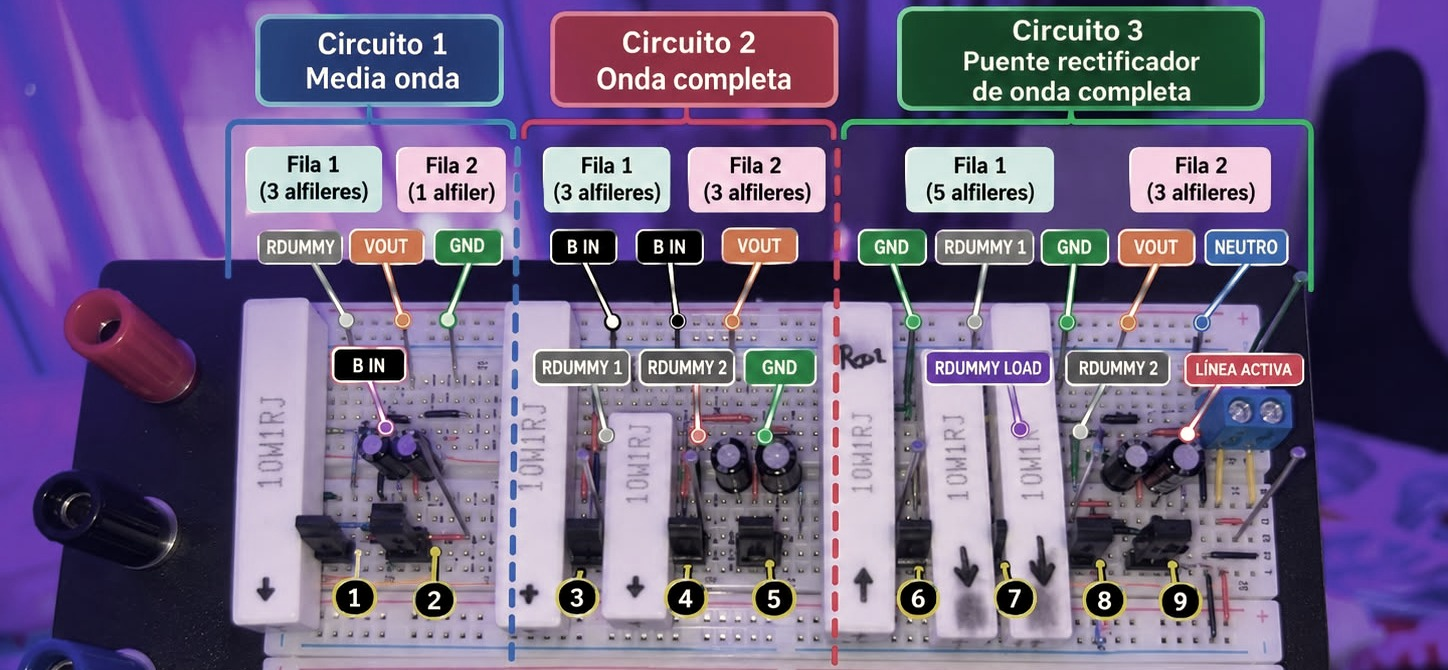
\includegraphics[width=0.9\textwidth]{sub_files/Imagenes/montaje.jpg}
  \caption{Montaje físico de los tres rectificadores con los switches SW$_1$ a SW$_9$ y los puntos de medición.}
  \label{fig:montaje}
\end{figure*}

% ---- Tablas de mediciones (C cerrado, A abierto, I izquierda, D derecha) --
\begin{table}[!t]
  \centering
  \footnotesize
  \caption{Mediciones del rectificador de media onda (C: cerrado, A: abierto, I: izquierda, D: derecha).}
  \label{tab:med_media}
  \begin{tabular}{llccl}
    \toprule
    \textbf{Carga} & \textbf{Medición} & \textbf{SW$_1$} & \textbf{SW$_2$} & \textbf{Archivo} \\ \midrule
    \multirow{2}{*}{$R_L$}               & $R_L$    & C & A & 1110.csv \\
                                         & $R_{D1}$ & A & A & 1120.csv \\ \midrule
    \multirow{2}{*}{$R_L \parallel C_1$} & $R_L$    & C & I & 1210.csv \\
                                         & $R_{D1}$ & A & I & 1220.csv \\ \midrule
    \multirow{2}{*}{$R_L \parallel C_2$} & $R_L$    & C & D & 1310.csv \\
                                         & $R_{D1}$ & A & D & 1320.csv \\ \bottomrule
  \end{tabular}
\end{table}

\begin{table}[!t]
  \centering
  \footnotesize
  \caption{Mediciones del rectificador de onda completa con tab central (C: cerrado, A: abierto, I: izquierda, D: derecha).}
  \label{tab:med_tab}
  \begin{tabular}{llcccl}
    \toprule
    \textbf{Carga} & \textbf{Medición} & \textbf{SW$_3$} & \textbf{SW$_4$} & \textbf{SW$_5$} & \textbf{Archivo} \\ \midrule
    \multirow{3}{*}{$R_L$}               & $R_L$    & C & C & A & 2110.csv \\
                                         & $R_{D3}$ & A & A & A & 2120.csv \\
                                         & $R_{D4}$ & A & A & A & 2130.csv \\ \midrule
    \multirow{3}{*}{$R_L \parallel C_1$} & $R_L$    & C & C & I & 2210.csv \\
                                         & $R_{D3}$ & A & A & I & 2220.csv \\
                                         & $R_{D4}$ & A & A & I & 2230.csv \\ \midrule
    \multirow{3}{*}{$R_L \parallel C_2$} & $R_L$    & C & C & D & 2310.csv \\
                                         & $R_{D3}$ & A & A & D & 2320.csv \\
                                         & $R_{D4}$ & A & A & D & 2330.csv \\ \bottomrule
  \end{tabular}
\end{table}

\begin{table}[!t]
  \centering
  \footnotesize
  \caption{Mediciones del puente rectificador (C: cerrado, A: abierto, I: izquierda, D: derecha).}
  \label{tab:med_puente}
  \begin{tabular}{llccccl}
    \toprule
    \textbf{Carga} & \textbf{Medición} & \textbf{SW$_6$} & \textbf{SW$_7$} & \textbf{SW$_8$} & \textbf{SW$_9$} & \textbf{Archivo} \\ \midrule
    \multirow{4}{*}{$R_L$}               & $R_L$    & C & C & C & A & 3110.csv \\
                                         & $R_{D6}$ & A & A & C & A & 3120.csv \\
                                         & $R_{D7}$ & A & A & C & A & 3130.csv \\
                                         & $R_{D8}$ & C & C & A & A & 3140.csv \\ \midrule
    \multirow{4}{*}{$R_L \parallel C_1$} & $R_L$    & C & C & C & I & 3210.csv \\
                                         & $R_{D6}$ & A & A & C & I & 3220.csv \\
                                         & $R_{D7}$ & A & A & C & I & 3230.csv \\
                                         & $R_{D8}$ & C & C & A & I & 3240.csv \\ \midrule
    \multirow{4}{*}{$R_L \parallel C_2$} & $R_L$    & C & C & C & D & 3310.csv \\
                                         & $R_{D6}$ & A & A & C & D & 3320.csv \\
                                         & $R_{D7}$ & A & A & C & D & 3330.csv \\
                                         & $R_{D8}$ & C & C & A & D & 3340.csv \\ \bottomrule
  \end{tabular}
\end{table}

% =====================================================================
% =====================================================================
%  Macros de los circuitos (CircuiTikZ ya se carga en el main con [american]).
%  Se puede \input en cualquier parte del documento antes de los circuitos.
% =====================================================================
% La convencion de voltaje RP va en cada circuito ([voltage dir=RP]) para no afectar otras figuras.

% ---- Etiquetas editables (cambiar con \renewcommand dentro de cada figura) ----
\providecommand{\etqFuente}{v_s}            % senal de entrada
\providecommand{\etqSec}{v_p}               % cada mitad del secundario (tab central)
\providecommand{\etqCarga}{R_L}             % resistencia de carga (reostato)
\providecommand{\etqSalida}{V_{out}}        % voltaje de salida
\providecommand{\etqCuno}{C_1}
\providecommand{\etqCdos}{C_2}
\providecommand{\etqRdummy}{1\,\Omega}      % valor de la R dummy
\providecommand{\sepCarga}{3.2}             % distancia R_L -> selector de C (subir si las etiquetas son largas)

% ---- Bloque: switch en paralelo con R dummy ----------------------------
% \dummyH{punto inicial}{largo}{switch}{resistencia}  horizontal, hacia la derecha
% \dummyV{punto inicial}{largo}{switch}{resistencia}  vertical, hacia abajo
\providecommand{\dummyH}[4]{%
  \draw (#1) to[short,*-] ++(0,0.6) to[nos, l={$#3$}] ++(#2,0) -- ++(0,-1.2)
             to[R, l={$#4$}] ++(-#2,0) -- ++(0,0.6);
  \draw (#1) ++(#2,0) node[circ]{};
}
\providecommand{\dummyV}[4]{%
  \draw (#1) to[short,*-] ++(-0.6,0) to[nos, l_={$#3$}] ++(0,-#2) -- ++(1.2,0)
             to[R, l_={$#4$}] ++(0,#2) -- ++(-0.6,0);
  \draw (#1) ++(0,-#2) node[circ]{};
}

% ---- Bloque: carga R_L con selector de capacitor en paralelo -----------
% \carga{nodo superior}{altura}{switch}
%   brazo al centro = abierto, izquierda = C1, derecha = C2
%   deja definida la coordenada (B) = nodo inferior de R_L
%   (flechas escritas como stealth-stealth para no chocar con babel-spanish)
\providecommand{\carga}[3]{%
  \coordinate (T) at (#1);
  \draw (T) to[vR, l_={$\etqCarga$}, v^={$\etqSalida$}, *-*] ++(0,-#2) coordinate(B);
  \draw (T) -- ++(\sepCarga,0) node[circ]{} coordinate(P) node[above]{$#3$};
  \draw[line width=0.8pt] (P) -- ++(0,-0.75);                          % brazo (abierto)
  \draw[stealth-stealth, thin] (P) ++(-125:0.55) arc[start angle=-125, end angle=-55, radius=0.55];
  \draw (P) ++(-0.7,-0.9) coordinate(K1) to[C, l_={$\etqCuno$}, o-*] (K1 |- B);
  \draw (P) ++( 0.7,-0.9) coordinate(K2) to[C, l={$\etqCdos$}, o-] (K2 |- B);
  \draw (B) -- (K2 |- B);
}

% ---- Transformador con tab central -------------------------------------
\providecommand{\trafoTab}{%
  \draw (0,0) to[sV, l={$\etqFuente$}] (0,4) -- (1.5,4) to[cute inductor] (1.5,0) -- (0,0);
  \draw[line width=1pt] (1.95,0.6) -- (1.95,3.4) (2.15,0.6) -- (2.15,3.4);
  \draw (2.6,4) to[cute inductor, mirror, l={$\etqSec$}] (2.6,2)
                to[cute inductor, mirror, l={$\etqSec$}] (2.6,0);
}


% ---- Bloques modulares -------------------------------------------------
\begin{figure*}[!t]
  \centering
  \subfloat[Switch en paralelo con $R_{D}$.\label{fig:bloque_dummy}]{%
    \resizebox{0.46\textwidth}{!}{% 4) Bloque: R dummy en paralelo con un switch
\begin{circuitikz}[voltage dir=RP]
  \draw (0,0) to[short,o-] (1,0);
  \dummyH{1,0}{2.4}{SW}{R_D = \etqRdummy}
  \draw (3.4,0) to[short,-o] (4.4,0);
  \node[right] at (5,0) {%
    \begin{tabular}{ll}
      \hline
      \textbf{SW} & \textbf{Resistencia vista} \\ \hline
      Cerrado & $0\,\Omega$ ($R_D$ en corto) \\
      Abierto & $R_D = \etqRdummy$ \\ \hline
    \end{tabular}};
\end{circuitikz}
}}
  \hfill
  \subfloat[Switch selector de capacitor en paralelo con $R_L$.\label{fig:bloque_carga}]{%
    \resizebox{0.50\textwidth}{!}{% 5) Bloque: carga R_L con switch selector de capacitor en paralelo
\begin{circuitikz}[voltage dir=RP]
  \draw (-1,2.8) to[short,o-] (0,2.8);
  \carga{0,2.8}{2.8}{SW}
  \draw (-1,0) to[short,o-] (B);
  \node[right] at (5.4,1.4) {%
    \begin{tabular}{ll}
      \hline
      \textbf{SW} & \textbf{Carga vista} \\ \hline
      Abierto   & $\etqCarga$ \\
      Izquierda & $\etqCarga \parallel \etqCuno$ \\
      Derecha   & $\etqCarga \parallel \etqCdos$ \\ \hline
    \end{tabular}};
\end{circuitikz}
}}
  \caption{Bloques modulares de los switches y su convención de estados.}
  \label{fig:bloques}
\end{figure*}

% ---- Circuitos adaptados ----------------------------------------------
\begin{figure*}[!t]
  \centering
  \subfloat[Media onda (SW$_1$, SW$_2$).\label{fig:adapt_media}]{%
    \resizebox{0.32\textwidth}{!}{% 6) Media onda adaptado: SW_1 (dummy entre R_L y tierra), SW_2 (selector de C)
\begin{circuitikz}[voltage dir=RP]
  \draw (0,0) to[sV, l={$\etqFuente$}] (0,5) to[D*, l=$D_1$] (3,5);
  \carga{3,5}{2.8}{SW_2}
  \dummyV{3,2.2}{2.2}{SW_1}{R_{D1}}
  \draw (0,0) -- (3,0);
  \draw (1.5,0) node[ground]{};
\end{circuitikz}
}}
  \hfill
  \subfloat[Onda completa con tab central (SW$_3$, SW$_4$, SW$_5$).\label{fig:adapt_tab}]{%
    \resizebox{0.62\textwidth}{!}{% 7) Tab central adaptado: SW_3 y SW_4 (dummies de cada rama), SW_5 (selector de C)
\begin{circuitikz}[voltage dir=RP]
  \trafoTab
  \draw (2.6,4) to[D*, l=$D_1$] (4.4,4) -- (4.8,4);
  \dummyH{4.8,4}{2.2}{SW_3}{R_{D3}}
  \draw (7,4) -- (8,4) -- (8,0);
  \draw (2.6,0) to[D*, l_=$D_2$] (4.4,0) -- (4.8,0);
  \dummyH{4.8,0}{2.2}{SW_4}{R_{D4}}
  \draw (7,0) -- (8,0);
  \draw (2.6,2) to[short,*-] (3.4,2) node[ground]{};
  \draw (8,2) to[short,*-] (9.6,2);
  \carga{9.6,2}{3.5}{SW_5}
  \draw (B) node[ground]{};
\end{circuitikz}
}}
  \\[2ex]
  \subfloat[Puente rectificador (SW$_6$ a SW$_9$).\label{fig:adapt_puente}]{%
    \resizebox{0.62\textwidth}{!}{% 8) Puente adaptado: dummies a tierra. SW_6 y SW_7 (ramas de diodos),
%    SW_8 (en serie con la carga), SW_9 (selector de C)
\begin{circuitikz}[voltage dir=RP]
  % ramas de diodos: la corriente sube desde tierra por la dummy y entra al anodo
  \dummyV{0,2.2}{2.2}{SW_6}{R_{D6}}
  \draw (0,2.2) to[D*, l=$D_2$] (0,4.4) to[D*, l=$D_1$] (0,6.6);
  \dummyV{4,2.2}{2.2}{SW_7}{R_{D7}}
  \draw (4,2.2) to[D*, l=$D_4$] (4,4.4) to[D*, l=$D_3$] (4,6.6);
  \draw (0,4.4) to[sV, l={$\etqFuente$}, *-*] (4,4.4);
  % carga y su dummy
  \draw (0,6.6) to[short,-*] (4,6.6) -- (8,6.6);
  \carga{8,6.6}{4.4}{SW_9}
  \dummyV{8,2.2}{2.2}{SW_8}{R_{D8}}
  % tierra
  \draw (0,0) -- (8,0);
  \draw (2,0) node[ground]{};
\end{circuitikz}
}}
  \caption{Circuitos adaptados con resistencias dummy y selector de capacitores.}
  \label{fig:adaptados}
\end{figure*}

% ---- Montaje fisico (va a proposito despues de los esquematicos que lo explican) --
\begin{figure*}[!t]
  \centering
  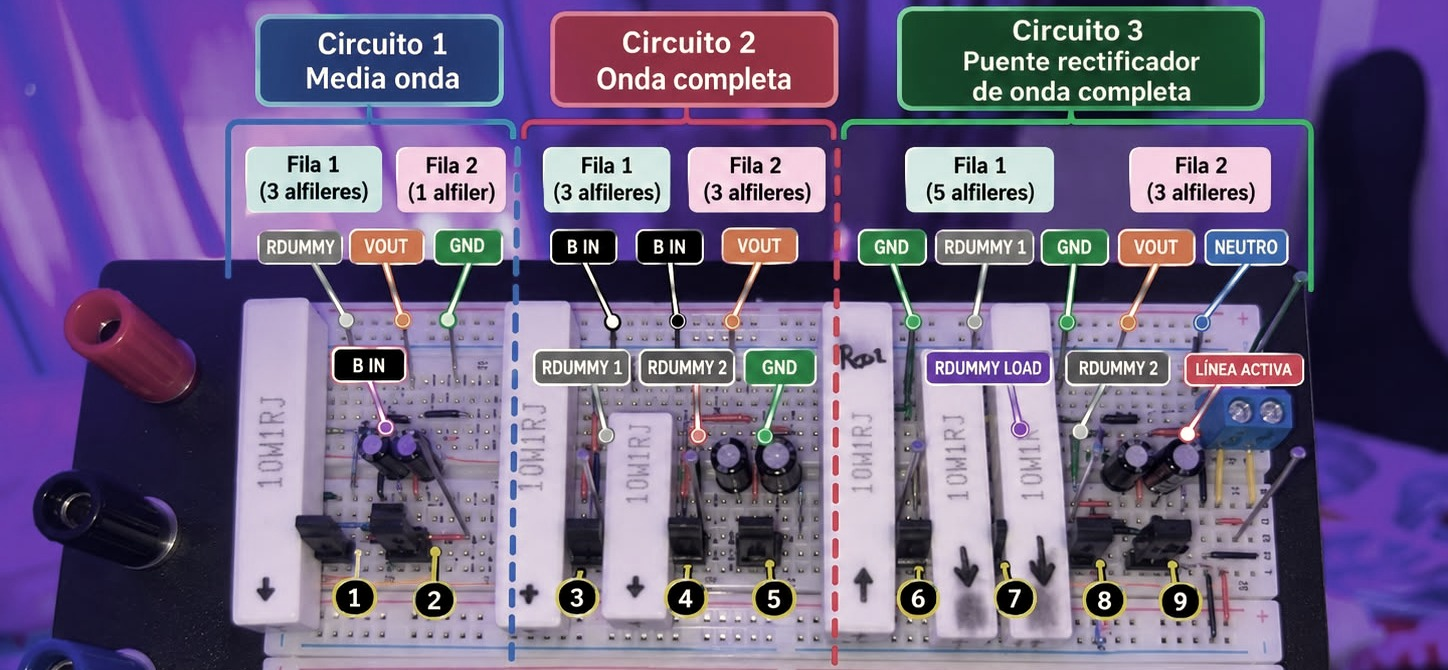
\includegraphics[width=0.9\textwidth]{sub_files/Imagenes/montaje.jpg}
  \caption{Montaje físico de los tres rectificadores con los switches SW$_1$ a SW$_9$ y los puntos de medición.}
  \label{fig:montaje}
\end{figure*}

% ---- Tablas de mediciones (C cerrado, A abierto, I izquierda, D derecha) --
\begin{table}[!t]
  \centering
  \footnotesize
  \caption{Mediciones del rectificador de media onda (C: cerrado, A: abierto, I: izquierda, D: derecha).}
  \label{tab:med_media}
  \begin{tabular}{llccl}
    \toprule
    \textbf{Carga} & \textbf{Medición} & \textbf{SW$_1$} & \textbf{SW$_2$} & \textbf{Archivo} \\ \midrule
    \multirow{2}{*}{$R_L$}               & $R_L$    & C & A & 1110.csv \\
                                         & $R_{D1}$ & A & A & 1120.csv \\ \midrule
    \multirow{2}{*}{$R_L \parallel C_1$} & $R_L$    & C & I & 1210.csv \\
                                         & $R_{D1}$ & A & I & 1220.csv \\ \midrule
    \multirow{2}{*}{$R_L \parallel C_2$} & $R_L$    & C & D & 1310.csv \\
                                         & $R_{D1}$ & A & D & 1320.csv \\ \bottomrule
  \end{tabular}
\end{table}

\begin{table}[!t]
  \centering
  \footnotesize
  \caption{Mediciones del rectificador de onda completa con tab central (C: cerrado, A: abierto, I: izquierda, D: derecha).}
  \label{tab:med_tab}
  \begin{tabular}{llcccl}
    \toprule
    \textbf{Carga} & \textbf{Medición} & \textbf{SW$_3$} & \textbf{SW$_4$} & \textbf{SW$_5$} & \textbf{Archivo} \\ \midrule
    \multirow{3}{*}{$R_L$}               & $R_L$    & C & C & A & 2110.csv \\
                                         & $R_{D3}$ & A & A & A & 2120.csv \\
                                         & $R_{D4}$ & A & A & A & 2130.csv \\ \midrule
    \multirow{3}{*}{$R_L \parallel C_1$} & $R_L$    & C & C & I & 2210.csv \\
                                         & $R_{D3}$ & A & A & I & 2220.csv \\
                                         & $R_{D4}$ & A & A & I & 2230.csv \\ \midrule
    \multirow{3}{*}{$R_L \parallel C_2$} & $R_L$    & C & C & D & 2310.csv \\
                                         & $R_{D3}$ & A & A & D & 2320.csv \\
                                         & $R_{D4}$ & A & A & D & 2330.csv \\ \bottomrule
  \end{tabular}
\end{table}

\begin{table}[!t]
  \centering
  \footnotesize
  \caption{Mediciones del puente rectificador (C: cerrado, A: abierto, I: izquierda, D: derecha).}
  \label{tab:med_puente}
  \begin{tabular}{llccccl}
    \toprule
    \textbf{Carga} & \textbf{Medición} & \textbf{SW$_6$} & \textbf{SW$_7$} & \textbf{SW$_8$} & \textbf{SW$_9$} & \textbf{Archivo} \\ \midrule
    \multirow{4}{*}{$R_L$}               & $R_L$    & C & C & C & A & 3110.csv \\
                                         & $R_{D6}$ & A & A & C & A & 3120.csv \\
                                         & $R_{D7}$ & A & A & C & A & 3130.csv \\
                                         & $R_{D8}$ & C & C & A & A & 3140.csv \\ \midrule
    \multirow{4}{*}{$R_L \parallel C_1$} & $R_L$    & C & C & C & I & 3210.csv \\
                                         & $R_{D6}$ & A & A & C & I & 3220.csv \\
                                         & $R_{D7}$ & A & A & C & I & 3230.csv \\
                                         & $R_{D8}$ & C & C & A & I & 3240.csv \\ \midrule
    \multirow{4}{*}{$R_L \parallel C_2$} & $R_L$    & C & C & C & D & 3310.csv \\
                                         & $R_{D6}$ & A & A & C & D & 3320.csv \\
                                         & $R_{D7}$ & A & A & C & D & 3330.csv \\
                                         & $R_{D8}$ & C & C & A & D & 3340.csv \\ \bottomrule
  \end{tabular}
\end{table}


%%%%%%%%%%%%%%%%%%%%%%%%%%%%%%%%%%%%%%%%%%%%%
\section{Resultados y Análisis}

En esta sección se presentan de forma consolidada las magnitudes teóricas calculadas, los resultados computacionales obtenidos en LTspice y los valores experimentales medidos en el banco de trabajo, acompañados del error relativo porcentual calculado mediante:
\begin{equation}
    \%\,\mathrm{Error} = \frac{|\mathrm{Medido} - \mathrm{Teórico}|}{\mathrm{Teórico}} \times 100\%
\end{equation}

% ==========================================
% TABLA 1 CONSOLIDADA: CARGA PURAMENTE RESISTIVA
% ==========================================
\begin{table*}[!t]
\centering
\small
\caption{Consolidado de resultados para carga puramente resistiva ($R = 220\,\Omega$).}
\label{tab:consolidado_tabla1}
\begin{tabular}{llcccccc}
\toprule
\textbf{Topología} & \textbf{Origen} & $\mathbf{V_{o-rms}}\,\mathrm{[V]}$ & $\mathbf{V_{o-DC}}\,\mathrm{[V]}$ & $\mathbf{V_{o-pico}}\,\mathrm{[V]}$ & $\mathbf{P}\,\mathrm{[W]}$ & $\mathbf{S}\,\mathrm{[VA]}$ & $\mathbf{PF}$ \\
\midrule
% ---------------- MEDIA ONDA ----------------
\textbf{Media onda} 
& Teórico   & 6.02  & 3.83  & 12.03 & 0.165 & 0.247 & 0.668 \\
& Simulado  &5.88 % <-- Escribe aquí tu dato de LTspice
& 3.68% <-- Vo-DC LTspice
& 11.94% <-- Vo-pico LTspice
& 0.157% <-- P LTspice
& 0.240% <-- S LTspice
& 0.668% <-- PF LTspice
\\
& Medido    & % <-- Dato del osciloscopio en el lab
& 
& 
& 
& 
& 
\\
& \% Error  & % <-- % Error
& 
& 
& 
& 
& 
\\
\midrule
% ---------------- TAP CENTRAL ----------------
\textbf{Tap central} 
& Teórico   & 8.51  & 7.66  & 12.03 & 0.329 & 0.493 & 0.667 \\
& Simulado  &8.53 % <-- LTspice
& 7.62
& 11.91
& 0.330
& 0.498
& 0.662
\\
& Medido    & % <-- Lab
& 
& 
& 
& 
& 
\\
& \% Error  & 
& 
& 
& 
& 
& 
\\
\midrule
% ---------------- PUENTE DE DIODOS ----------------
\textbf{Puente de diodos} 
& Teórico   & 17.01 & 15.32 & 24.06 & 1.315 & 1.391 & 0.945 \\
& Simulado  &16.53 % <-- LTspice
& 14.63
& 23.74
& 1.23
& 1.35
& 0.91
\\
& Medido    & % <-- Lab
& 
& 
& 
& 
& 
\\
& \% Error  & 
& 
& 
& 
& 
& 
\\
\bottomrule
\end{tabular}
\end{table*}

% ==========================================
% TABLA 2 CONSOLIDADA: CARGA RC CON FILTRO
% ==========================================
\begin{table*}[!t]
\centering
\small
\caption{Consolidado de resultados para carga con filtro capacitivo ($R = 220\,\Omega$).}
\label{tab:consolidado_tabla2}
\begin{tabular}{lllccccc}
\toprule
\textbf{Topología} & $\mathbf{C_{\mathrm{filtro}}}$ & \textbf{Origen} & $\mathbf{V_{o-rms}}\,\mathrm{[V]}$ & $\mathbf{V_{o-DC}}\,\mathrm{[V]}$ & $\mathbf{V_{o-pico}}\,\mathrm{[V]}$ & $\mathbf{FR}\,[\%]$ & $\mathbf{PF}$ \\
\midrule
% ---------------- MEDIA ONDA (BAJO RIZO) ----------------
\textbf{Media onda} & \multirow{4}{*}{$220\,\mu\mathrm{F}$} 
& Teórico   & 10.0  & 9.9   & 12.0  & 9.9\% & 0.35 \\
($FR < 10\%$) & & Simulado  &10.34 &10.3 &11.82 &9.29\% &0.38 \\
              & & Medido    & & & & & \\
              & & \% Error  & & & & & \\
\cmidrule(lr){2-8}
% ---------------- MEDIA ONDA (ALTO RIZO) ----------------
\textbf{Media onda} & \multirow{4}{*}{$47\,\mu\mathrm{F}$} 
& Teórico   & 6.9   & 6.4   & 12.0  & 46.5\% & 0.52 \\
($FR > 30\%$) & & Simulado  &7.77 &7.30 &11.90 &37.12\% &0.45 \\
              & & Medido    & & & & & \\
              & & \% Error  & & & & & \\
\midrule
% ---------------- TAP CENTRAL (BAJO RIZO) ----------------
\textbf{Tap central} & \multirow{4}{*}{$220\,\mu\mathrm{F}$} 
& Teórico   & 11.0  & 11.0  & 12.0  & 5.0\% & 0.40 \\
($FR < 10\%$) & & Simulado  &11.1 &11.09 &11.83 &3.99\% &0.29 \\
              & & Medido    & & & & & \\
              & & \% Error  & & & & & \\
\cmidrule(lr){2-8}
% ---------------- TAP CENTRAL (ALTO RIZO) ----------------
\textbf{Tap central} & \multirow{4}{*}{$33\,\mu\mathrm{F}$} 
& Teórico   & 9.6   & 9.2   & 12.0  & 33.1\% & 0.55 \\
($FR > 30\%$) & & Simulado  &9.28 &9.07 &11.90 &23.22\% &0.33 \\
              & & Medido    & & & & & \\
              & & \% Error  & & & & & \\
\midrule
% ---------------- PUENTE (BAJO RIZO) ----------------
\textbf{Puente} & \multirow{4}{*}{$220\,\mu\mathrm{F}$} 
& Teórico   & 22.0  & 22.0  & 24.1  & 5.0\% & 0.58 \\
($FR < 10\%$) & & Simulado  &21.95 &21.93 &23.44 &4.01\% &0.63 \\
              & & Medido    & & & & & \\
              & & \% Error  & & & & & \\
\cmidrule(lr){2-8}
% ---------------- PUENTE (ALTO RIZO) ----------------
\textbf{Puente} & \multirow{4}{*}{$33\,\mu\mathrm{F}$} 
& Teórico   & 19.3  & 18.5  & 24.1  & 33.1\% & 0.72 \\
($FR > 30\%$) & & Simulado  &18.50 &18.09 &23.75 &23.23\% &0.65 \\
              & & Medido    & & & & & \\
              & & \% Error  & & & & & \\
\bottomrule
\end{tabular}
\end{table*}
%%%%%%%%%%%%%%%%%%%%%%%%%%%%%%%


%%%%%%%%%%%%%%%%%%%%%%%%%%%%%%%
%%%%%%%%Resultados y analsis y conclusiones en p2.tex%%%%%%%%%

    %%%%%%%%%%%%%%%%%%%%%%%%%%%%%%%%%%%%%%%%%%%%%%%%%%%%%%%%%%%%%%%%%%%%%%%%%%%%%%%%%%%%%%%%%%%%%


%\begin{table*}[t]
%\centering
%\caption{Bill of Materials (BOM)}
%\label{tab:bom}
%\renewcommand{\arraystretch}{1.3}
%\begin{tabular}{|c|c|l|l|c|}
%\hline
%\multicolumn{5}{|c|}{\textbf{Componentes Electrónicos (BOM)}} \\ \hline
%\textbf{Ítem} & \textbf{Cant.} & \textbf{Componente} & \textbf{Valor / Descripción} & \textbf{Designador} \\ \hline
%1 & 5 & Circuito Integrado Op-Amp & LM741CN (Entradas BJT) & U1 \\ \hline
%2 & 2 & Resistencia (5 W, 5\%) & $6.8 \text{ k}  \ \Omega$ & R1 \\ \hline
%3 & 3 & Resistencia (1/4 W, 5\%) & $1 \text{ k}\Omega$ & R2 \\ \hline
%4 & 3 & Resistencia (1/4 W, 5\%) & $5.6 \text{ k}\Omega$ & R3 \\ \hline
%5 & 1 & Resistencia (1/4 W, 5\%) & $20 \text{k}\Omega$ & R4 \\ \hline
%6 & 2 & Resistencia (1/4 W, 5\%) & $10 \text{k}\Omega$ & R5 \\ \hline
%7 & 2 & Resistencia (1/4 W, 5\%) & $2.2 \text{k}\Omega$ & R6 \\ \hline
%8 & 2 & Resistencia (1/4 W, 5\%) & $2.7 \text{k}\Omega$ & R7 \\ \hline
%9 & 1 & Resistencia (1/4 W, 5\%) & $1.2 \text{k}\Omega$ & R8 \\ \hline
%10 & 2 & Resistencia (1/4 W, 5\%) & $560 \text{}\Omega$ & R9 \\ \hline
%11 & 6 & Condensador cerámico & $12 \ \text{nF}$ ($\geq 25\text{V}$) & C1, C2 \\ \hline
%12 & 2 & Condensador Cerámico & $10n \ \text{F}$ & C3 \\ \hline
%13 & 1 & Condensador Cerámico & $24n \ \text{F}$ & C3 \\ \hline
%14 & 1 & Protoboard & Estándar para prototipado & - \\ \hline
%15 & 1 & Cables de conexión & Cables para protoboard & - \\ \hline
%\end{tabular}
%\end{table*}


%------------------------------------------------------------------------
%------------------------------------------------------------------------
%------------------------------------------------------------------------
    % Figuras y analisis correspondientes a Resultados y analisis.



\section{Conclusiones}

    \bibliographystyle{IEEEtran}
    \bibliography{referencias}
    %%%%%%%%%%%%%%%%%%%%%%%%%%%%%%%%%%%%%%%%%%%%%%%%%%%%%%%%%%%%%%%%%%%%%%%%%%%%%%%%








% --------------------------------------------------------------------------- %
% --------------------------------------------------------------------------- %
% --------------------------------------------------------------------------- %
% --------------------------------------------------------------------------- %
% --------------------------------------------------------------------------- %
\end{document}
    
    
